\chapter{\acrshort{ux} \& \acrshort{ui} design} \label{chapter4}

Because our survey indicated that we need to pay special attention to designing the interface of our application (see section \ref{3:appearance}), we decided to take an iterative approach to defining the \acrlong{ux} (\acrshort{ux}), and, by extension, sketching the \acrlong{ui} (\acrshort{ui}).

\section{Requirements} \label{4:requirements}

The proposed functionalities of our application are listed in section \ref{1:functionalities}. We will aim to reach our goals, as described in section \ref{1:goals}.

We will be designing a collaborative application (a decision motivated in section \ref{2:mix_and_match}) with a moderation system based on permission levels, described in this chapter in section \ref{4:permissions}.

Based on the results of our survey (section \ref{3:appearance}), our design language of choice will be neither Google's Material Design\cite{google2020material}, nor Apple's Human Interface Guidelines\cite{apple2020human}, but rather what we consider to be a healthy mix of both. This design aims to be easy on the eyes of both Android and iOS users, as is required of a cross-platform application which aims to have a consistent design on all platforms. A good example of another such application is \textit{Reddit} (available on both the App Store\footnote{https://apps.apple.com/us/app/reddit/id1064216828} and Google Play\footnote{https://play.google.com/store/apps/details?id=com.reddit.frontpage} with a very similar design that only slightly differs in the web version\footnote{http://reddit.com/}). However, since it sports a platform-agnostic design, independent developers have come up with separate applications for viewing \textit{Reddit} content on Android and iOS devices which claim to have a more "native" look for the more nitpicky users. A visual comparison between these applications can be seen in appendix \ref{a:native_cross}.

\section{Paper prototyping} \label{4:paper}

\subsection{Initial concept} \label{4:paper_concept}

We kick-started the design process by making a rough sketch of what we were imagining the app to look like, on paper, with the features we had in mind in the beginning. We used the \textit{School Assistant} app (see section \ref{2:generic_apps}) as the main inspiration for this first design.

\begin{figure}[ht]
    \centering
         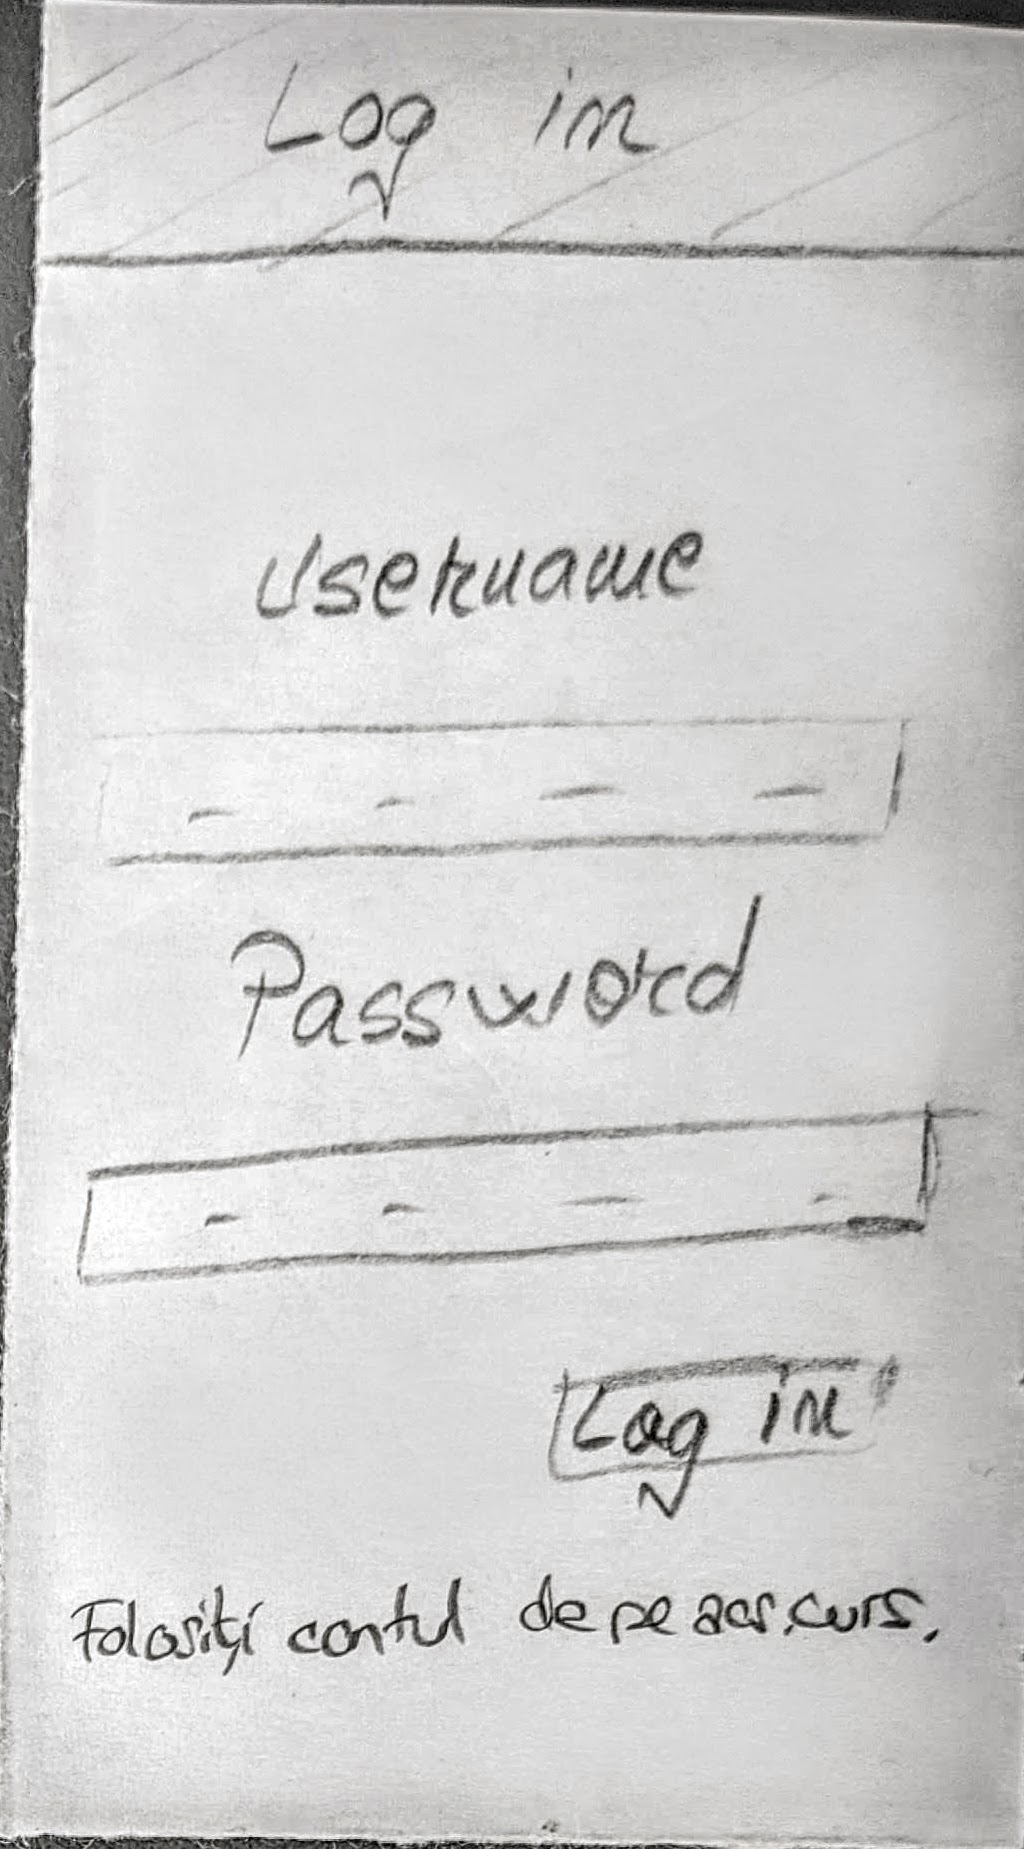
\includegraphics[height=0.279\textheight]{figures/app/paper/login.jpg}
         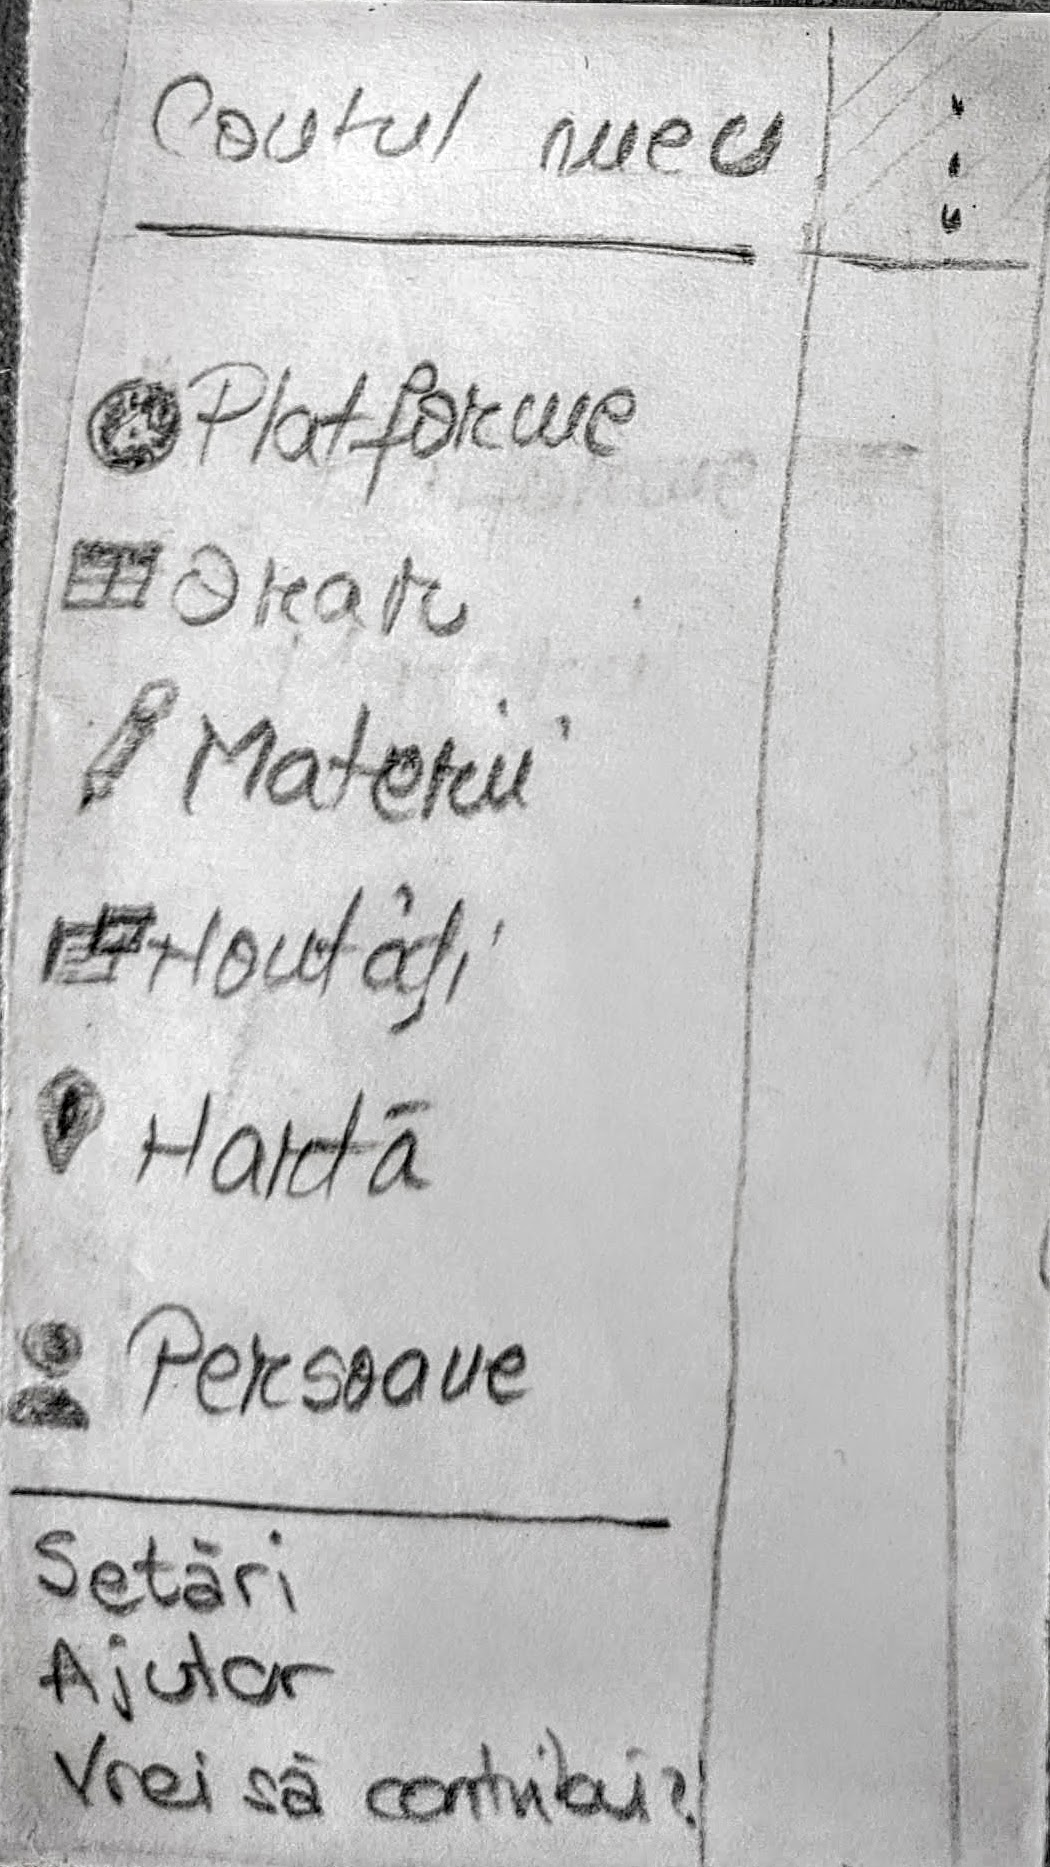
\includegraphics[height=0.279\textheight]{figures/app/paper/drawer.jpg}
         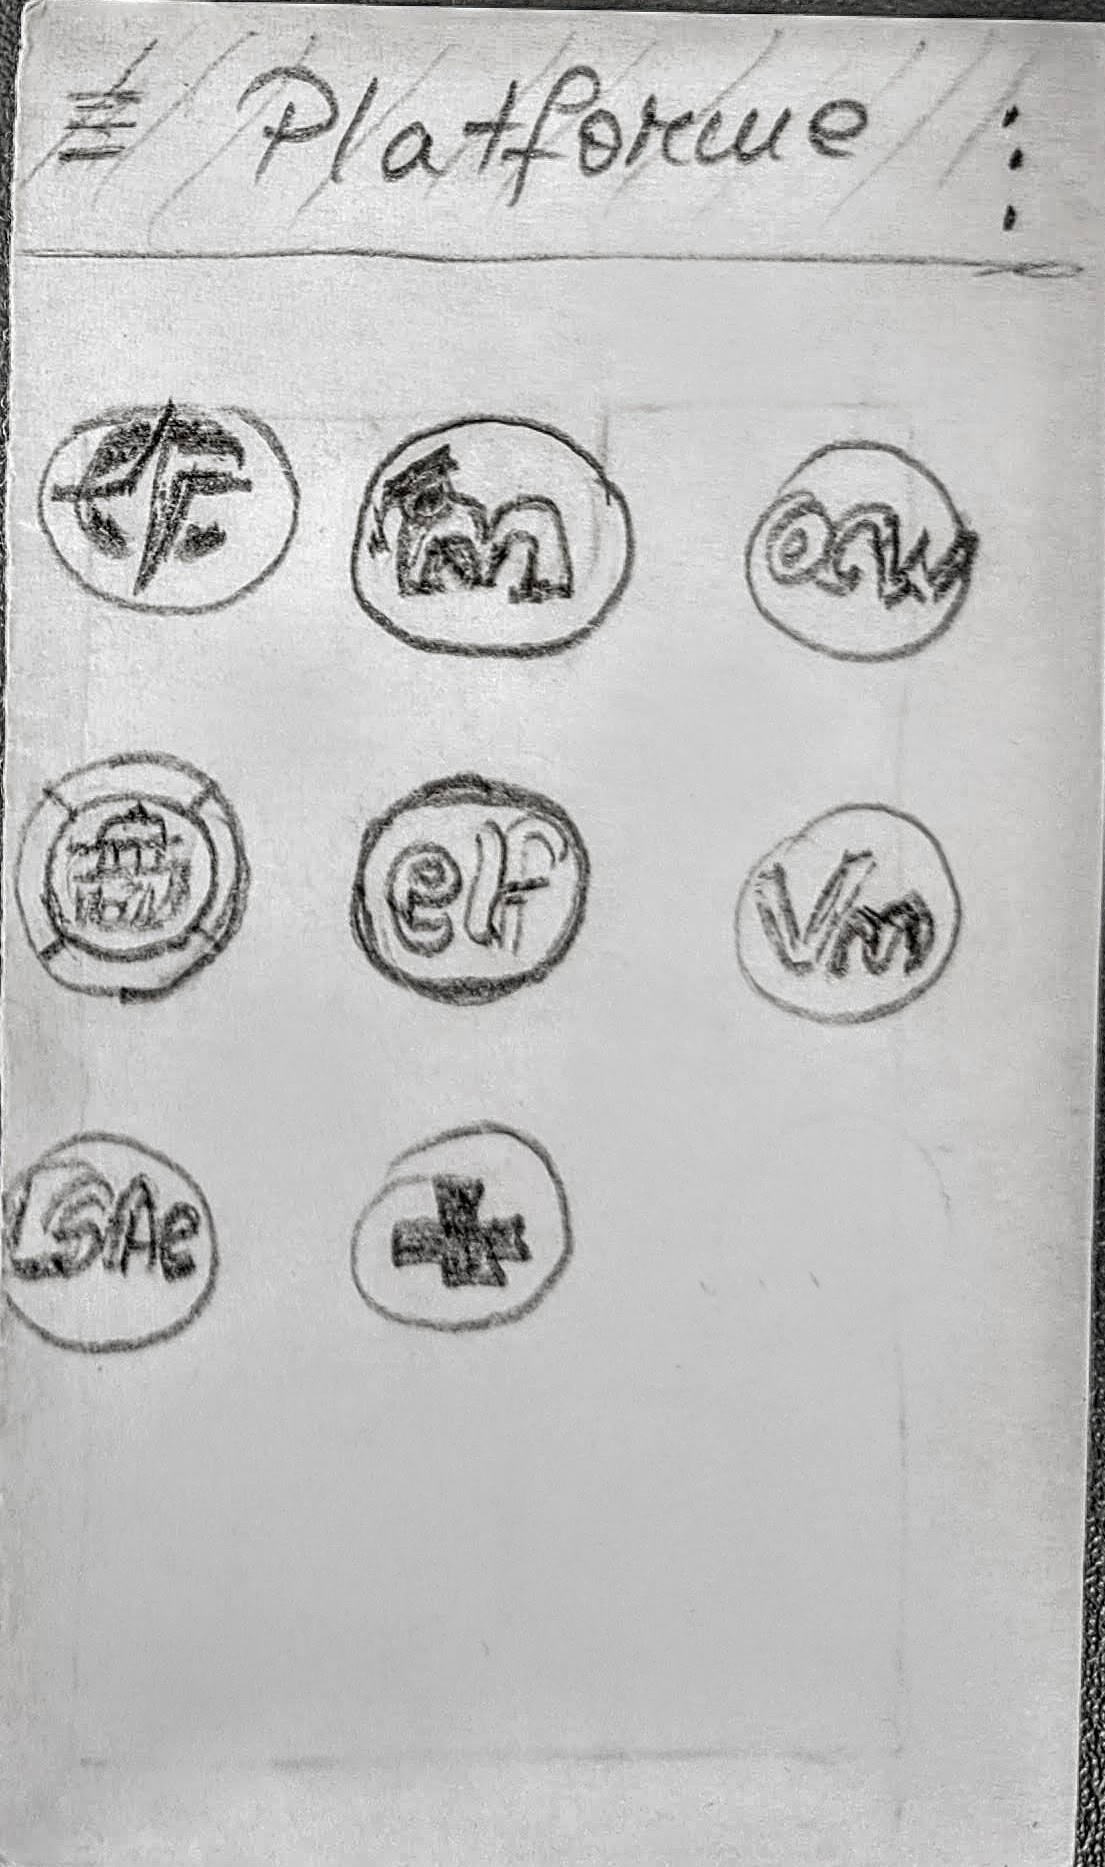
\includegraphics[height=0.279\textheight]{figures/app/paper/platforms.jpg}
         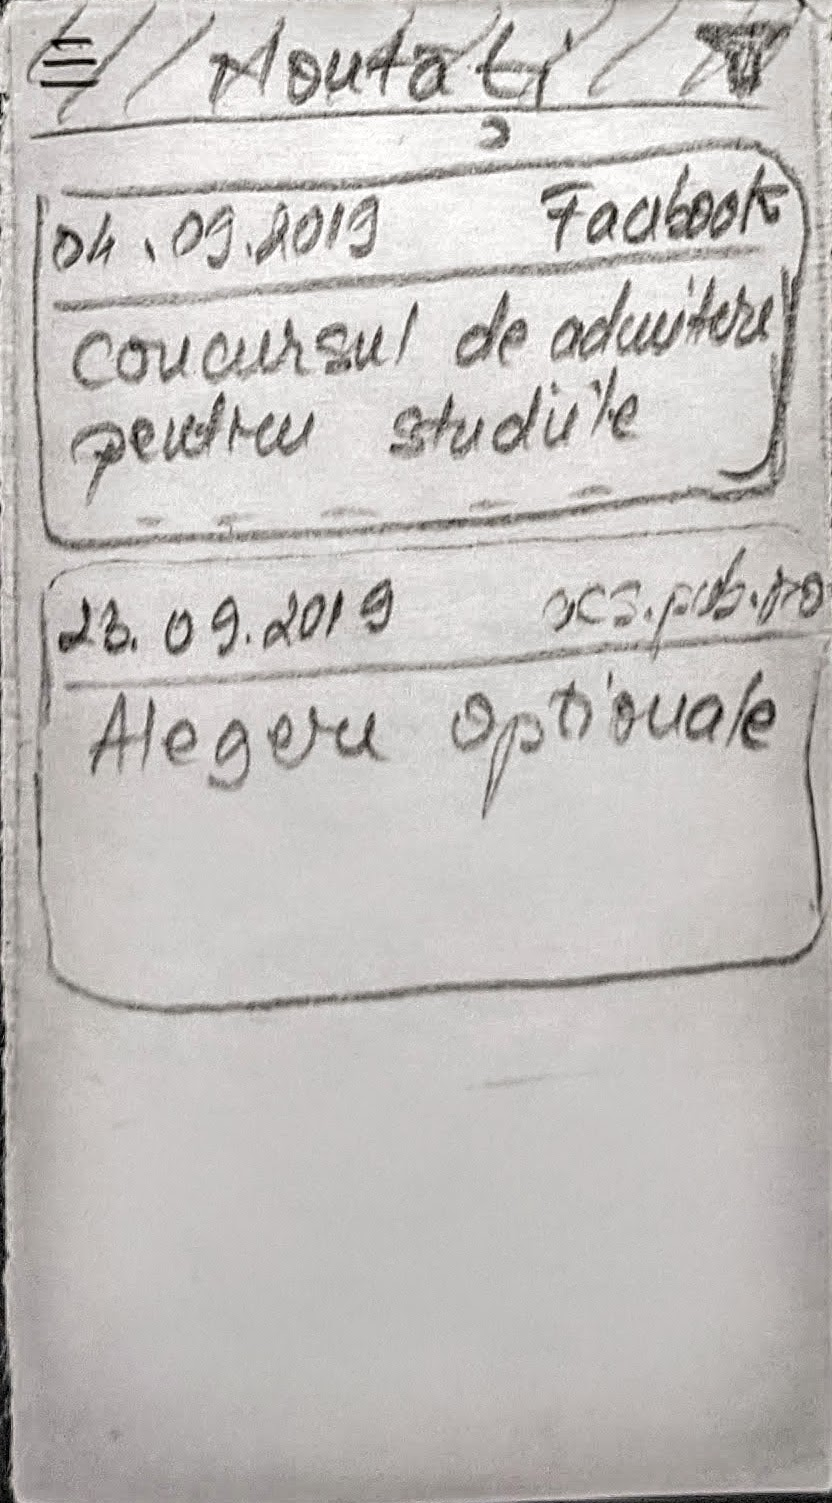
\includegraphics[height=0.279\textheight]{figures/app/paper/news.jpg}
         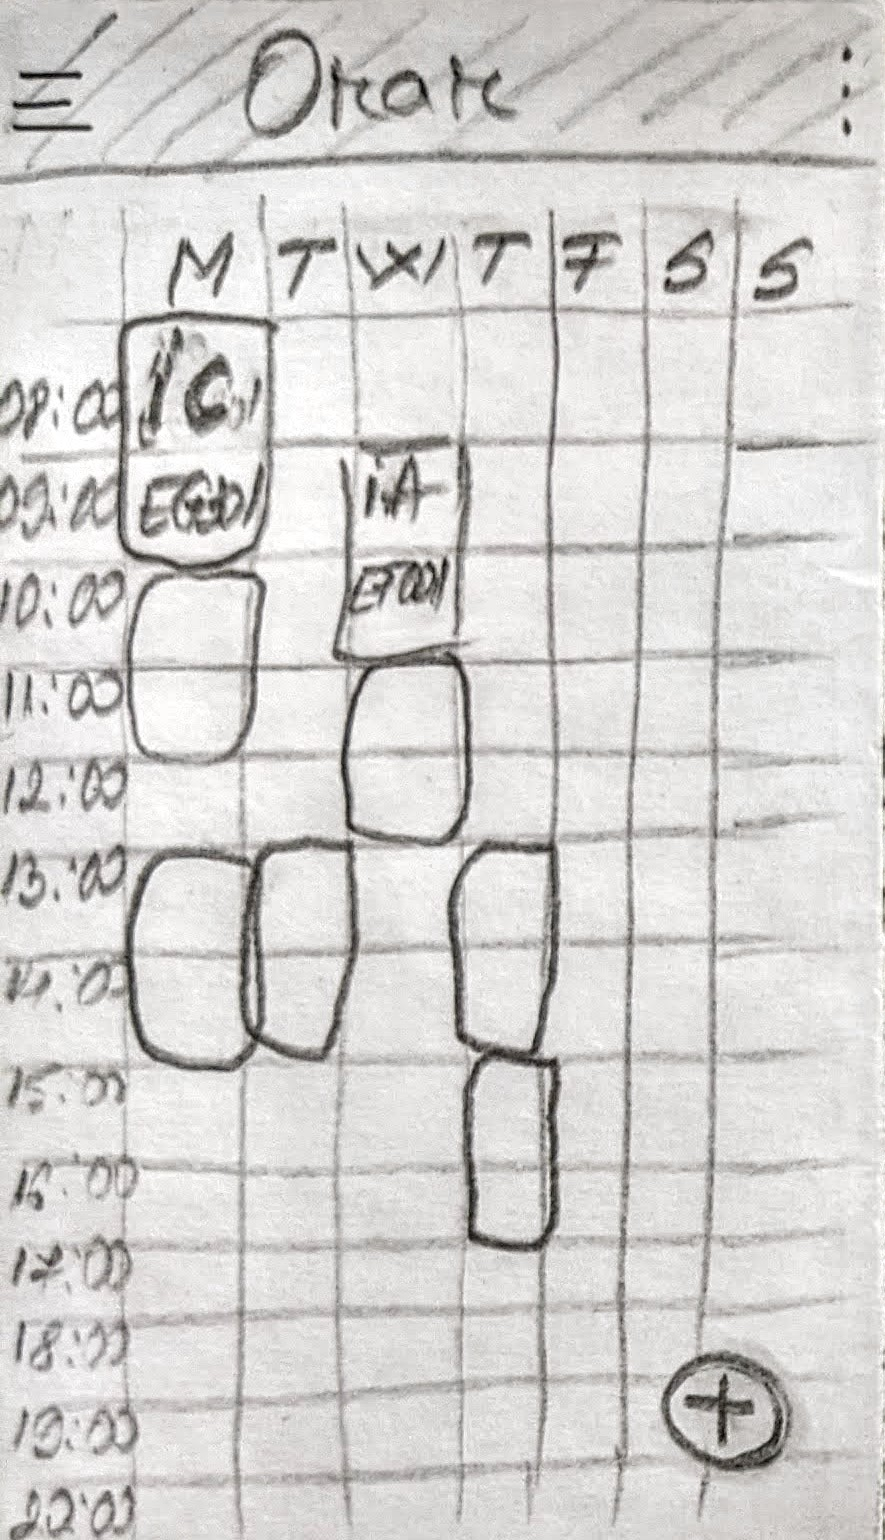
\includegraphics[height=0.279\textheight]{figures/app/paper/timetable.jpg}
         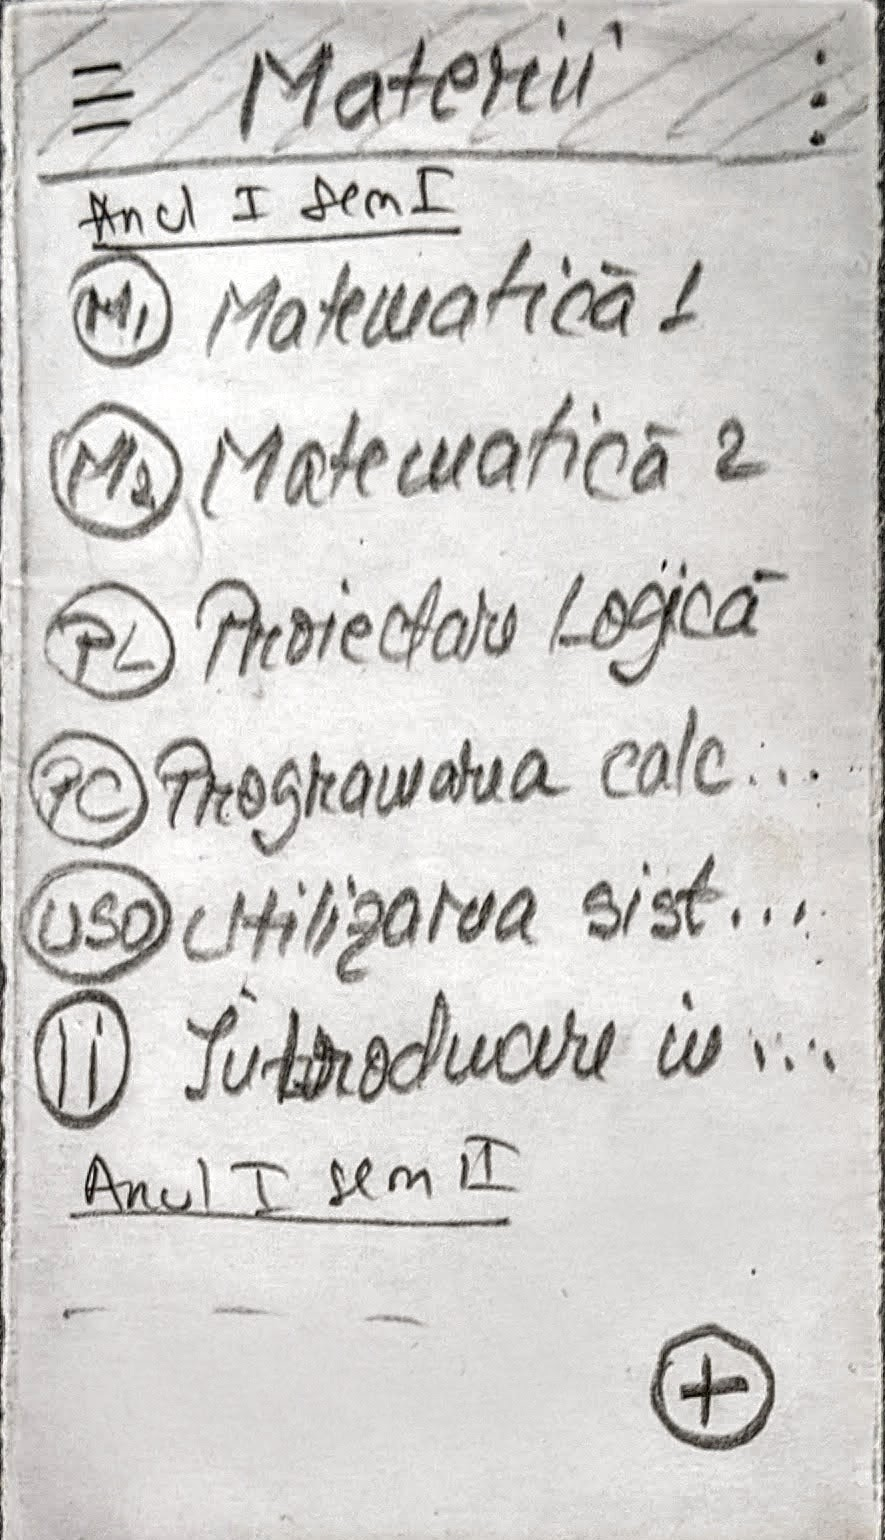
\includegraphics[height=0.279\textheight]{figures/app/paper/classes.jpg}
         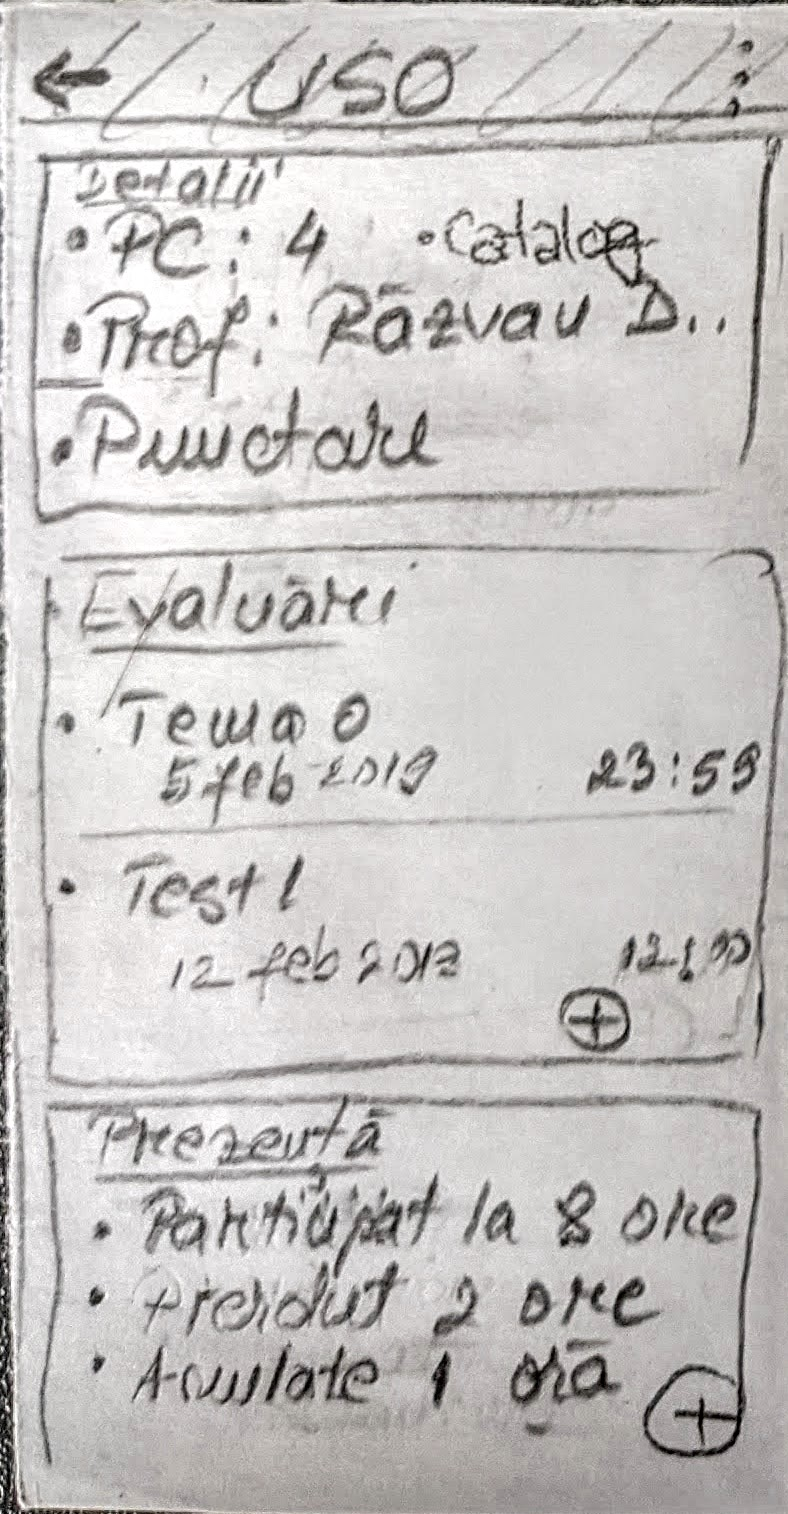
\includegraphics[height=0.279\textheight]{figures/app/paper/class_info.jpg}
         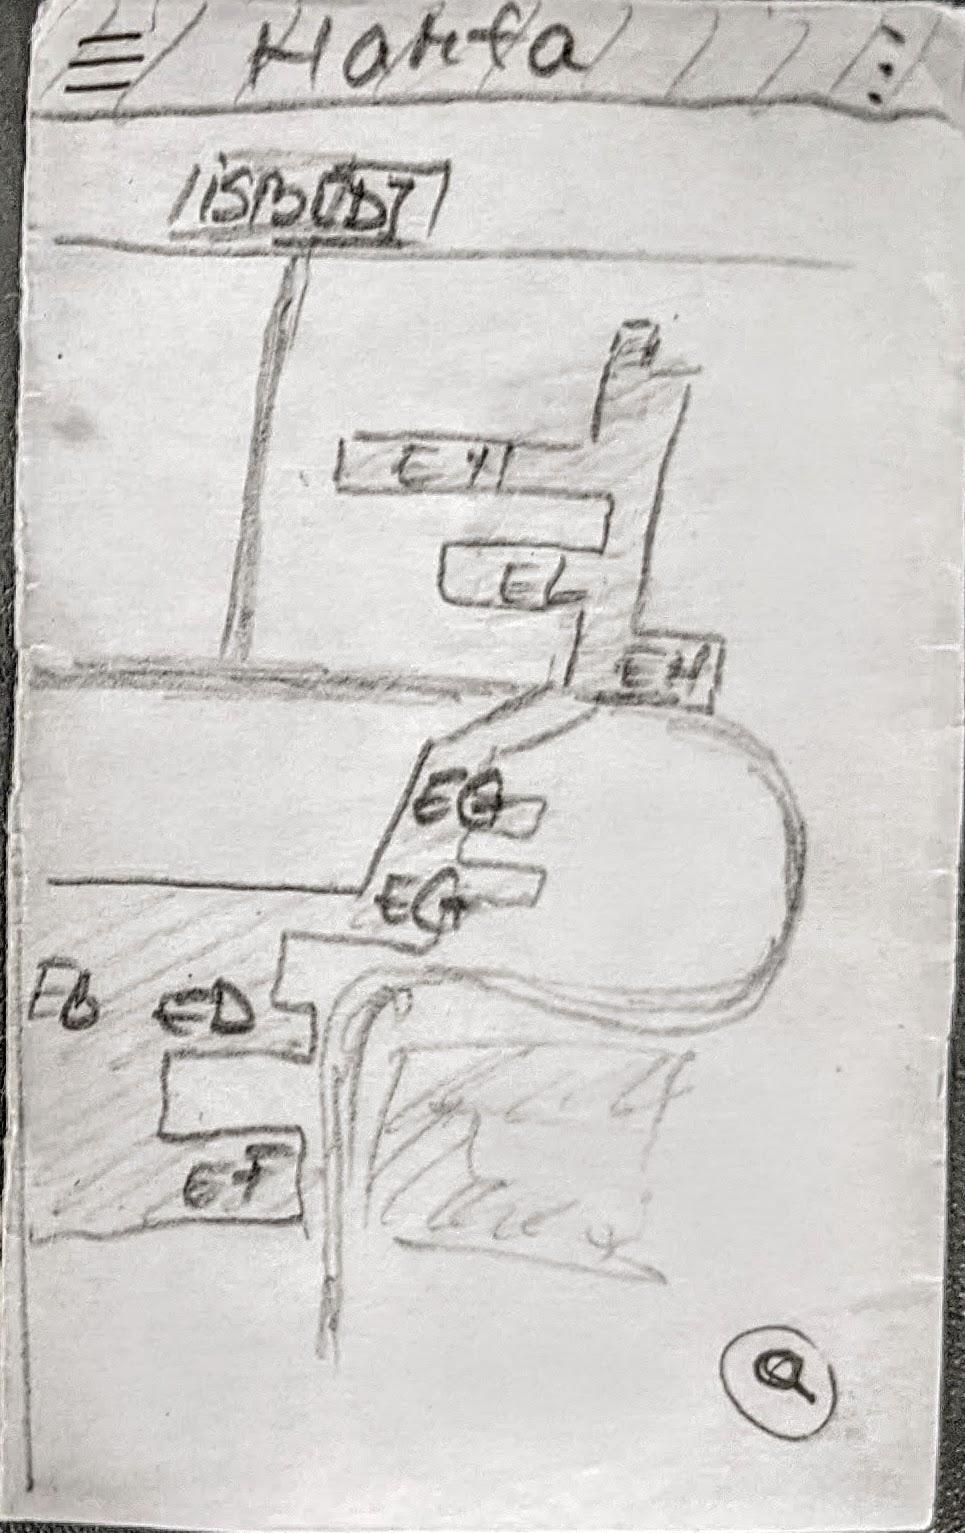
\includegraphics[height=0.279\textheight]{figures/app/paper/map.jpg}
    \caption{Paper prototype}
    \label{4:fig:paper_prototyping}
\end{figure}

\clearpage

Figure \ref{4:fig:paper_prototyping} shows the very first sketches of the application interface. The pages pictured, from left to right and top to bottom, are:
\begin{itemize}
    \setlength{\topsep}{0.5pt}
    \setlength{\itemsep}{0.5pt}
    \setlength{\parsep}{0.5pt}
    \item the login page the user would see when first opening the app
    \item the Material\cite{google2020material}-style side drawer with the different pages in the app, available once the user logs in
    \item the list of platforms provided by the university, which would serve as the default page the user would see without accessing the drawer
    \item the "News" page with information from various sources, such as relevant Facebook pages and the official website
    \item the timetable, with a button to add a new event
    \item the list of classes, organised by year/semester, with a button to add a new class
    \item information about a class, that a user would see when clicking on an event in the timetable or a class in the list
    \item the map of the campus, with a button to search for a specific location
\end{itemize}

\subsection{Feedback} \label{4:paper_feedback}

In order to find out what students would think about this initial concept, we organised a focus group with about 15 students and presented each of them the workflow of our application. Regarding \textbf{authentication}, we have received feedback about the need of a profile page for the user, as well as the possibility for a user to use the app without having to authenticate. Multiple students pointed out that having the "Platforms" page as the default was counter-intuitive, and that a \textbf{designated "Home" page} would be a better solution. When asked what they think this homepage should contain, they suggested quick actions and upcoming events, in other words an overview at a glance of the other pages within the app.

Some students pointed out that the homework-type events should have both \textbf{a soft and a hard deadline} associated with them, as is the norm in the faculty. Additionally, they wanted to see how the process of adding a new event would work.

\section{Permissions \& moderation system} \label{4:permissions}

\subsection{The need for moderation} \label{4:permissions_need}

As mentioned in section \ref{2:mix_and_match}, any collaborative system involving more than a few users requires some form of moderation\cite{roberts2019behind}. This is meant to ensure that content stays accurate and up-to-date, as well as avoid offensive/inappropriate content.

Based on the categories described by a \textit{Bridged.co} writer\cite{bridged2019moderation}, we will be using a mixture of \textbf{pre-moderation} and \textbf{reactive moderation}, meaning that content will be verified before appearing on the platform, and users can report or flag content that they believe to be inappropriate after it has been posted.

\subsection{Permission levels} \label{4:permissions_levels}

Since the platform should eventually be self-sustainable, without the need of constant involvement from the developer in content moderation (as is the case for the nonscalable solution of the application \textit{Politehnik}, described in section \ref{2:existing_apps_timetable}), we need a way to offer students the ability to moderate content on the platform themselves. This begs the question - how do we decide who should have the right to moderate content, and who should not?

In order to establish who should have certain rights, we first need to define the rights that are to be granted. We have designed a permission-level system, where each user has a permission number which indicates what they can do within the application:

\begin{itemize}
    \setlength{\topsep}{0.5pt}
    \setlength{\itemsep}{0.5pt}
    \setlength{\parsep}{0.5pt}
    \item TODO
\end{itemize}

\section{Wireframe} \label{4:wireframe}

\subsection{Prototype} \label{4:wireframe_prototype}

\subsection{Feedback} \label{4:wireframe_feedback}

\section{Final design} \label{4:final}